\section*{Klassediagram\label{klassediagram}}
I dette afsnit vil vi kort gennemg�r vores klassediagram. Diagrammet har et s�dan omfang at vi har v�ret n�d til at dele det op i mindre bidre, dels for at g�re det muligt at l�se og dels for at skabe overblik.

Gennem af entitetsklasserne vil blive gennemg�et oppe fra og ned. �verst oppe har en kontainer som indeholder en m�ngde 'Sessioner'. En 'Session' har en m�ngde af 'kunder' som opbevaret i klassen 'KundeKontainer'. En 'Kunde' har tilknyttet sig fire kontainere, som hveris�r best�r af 'Intaegter', 'Aktiver', 'Passiver' og 'Pensioner'. Ovenst�ende beskrivelse kan ses p� figur \ref{Klassediagramhoved} p� side \pageref{Klassediagramhoved}.

\begin{figure}
\begin{center}
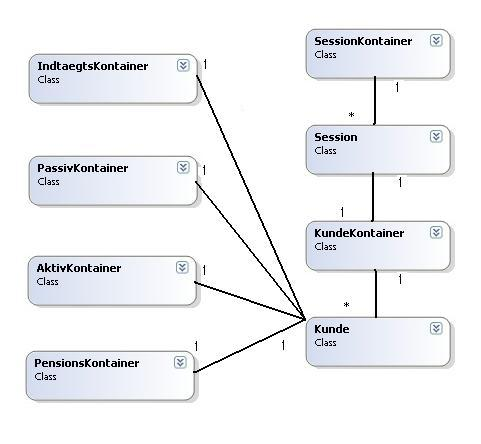
\includegraphics[width=1.0\textwidth]{Billeder/Klassediagram/ClassDiagramHoved.jpg} 
\end{center}
\caption{Klassediagram, Entiteter}
\label{Klassediagramhoved}
\end{figure}

De fire n�ste klassediagrammer viser forholdet mellem en kontainer klasser og den klasse som den er kontainer for. De viser ogs� hvorledes af vi har gjort brug af arv. Diagram \ref{fig:ClassDiagramIndtaegt} kan ses p� side \pageref{fig:ClassDiagramIndtaegt}, \ref{fig:ClassDiagramAktiv} kan ses p� side \pageref{fig:ClassDiagramAktiv}, 
\ref{fig:ClassDiagramPassiv} kan ses p� side \pageref{fig:ClassDiagramPassiv} og \ref{fig:ClassDiagramPension} kan ses p� side \pageref{fig:ClassDiagramPension}.

\begin{figure}
	\centering
		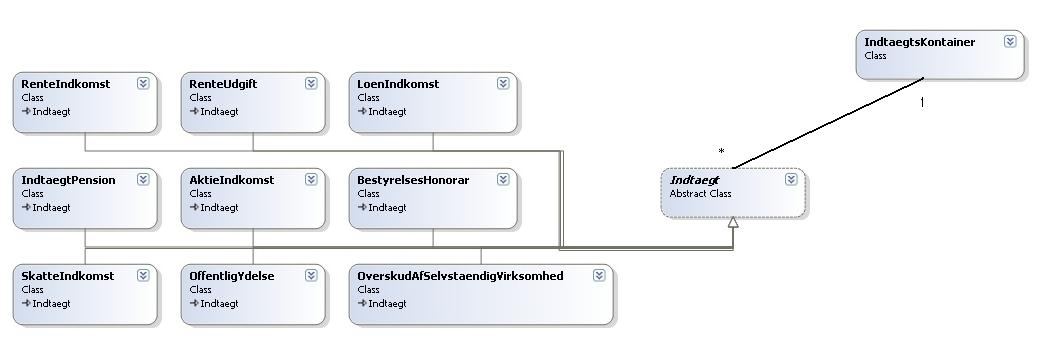
\includegraphics[width=1.00\textwidth]{Billeder/Klassediagram/ClassDiagramIndtaegt.jpg}
	\caption{Klassediagram, Int�gter}
	\label{fig:ClassDiagramIndtaegt}
\end{figure}

\begin{figure}
	\centering
		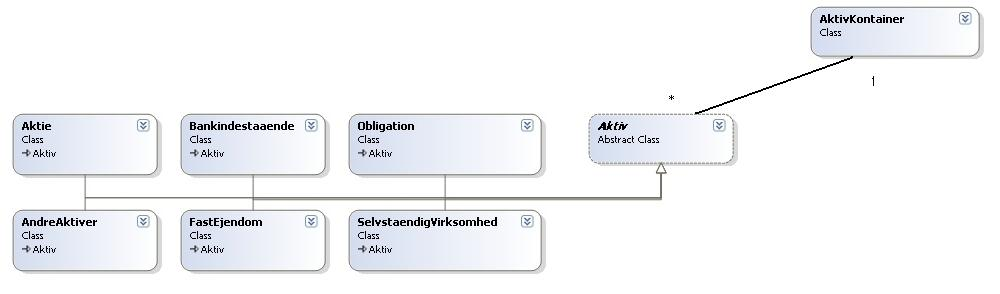
\includegraphics[width=1.00\textwidth]{Billeder/Klassediagram/ClassDiagramAktiv.jpg}
	\caption{Klassediagram, Aktiver}
	\label{fig:ClassDiagramAktiv}
\end{figure}

\begin{figure}
	\centering
		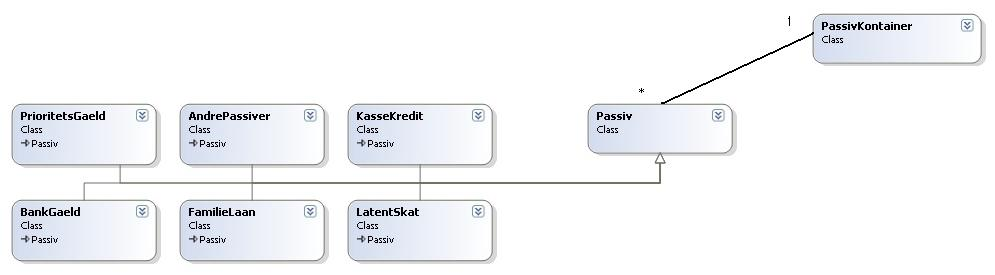
\includegraphics[width=1.00\textwidth]{Billeder/Klassediagram/ClassDiagramPassiv.jpg}
	\caption{Klassediagram, Passiver}
	\label{fig:ClassDiagramPassiv}
\end{figure}

\begin{figure}
	\centering
		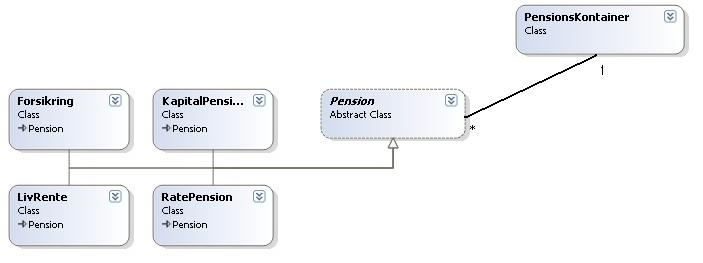
\includegraphics[width=1.00\textwidth]{Billeder/Klassediagram/ClassDiagramPension.jpg}
	\caption{Klassediagram, Pensioner}
	\label{fig:ClassDiagramPension}
\end{figure}

Efterf�lgende var vi et diagram som viser at der en 'kontrol' klasse som hver styer mellem 1 og 3 forme/skr�me. Dette repr�sentere kontrol og view i design patternet MVC, som der kan l�se om i afsnit \ref{MVC} p� side \pageref{MVC}.

\begin{figure}
	\centering
		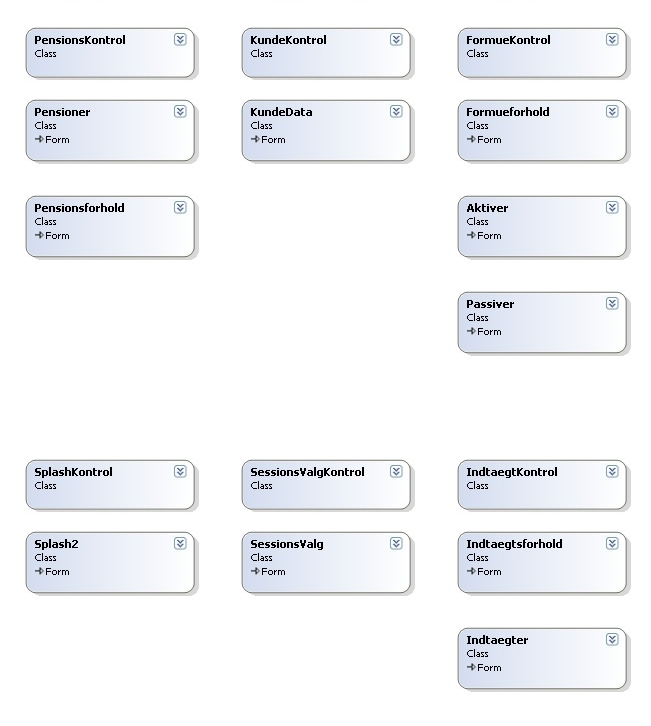
\includegraphics[width=1.00\textwidth]{Billeder/Klassediagram/ClassDiagramGuiKontrol.jpg}
	\caption{Klassediagram, Kontrol, View}
	\label{fig:ClassDiagramGuiKontrol}
\end{figure}

Det sidste klassediagram vi kan byde p� indeholde forskellige klasser. Dette hendler om klassen der tager sig af at kommunikere be databasen, vores post nr. klasse og to klasser som kan bruges til at sortere med. Diagram \ref{fig:ClassDiagramMiscdetaile} kan ses \pageref{fig:ClassDiagramMiscdetaile}.

\begin{figure}
	\centering
		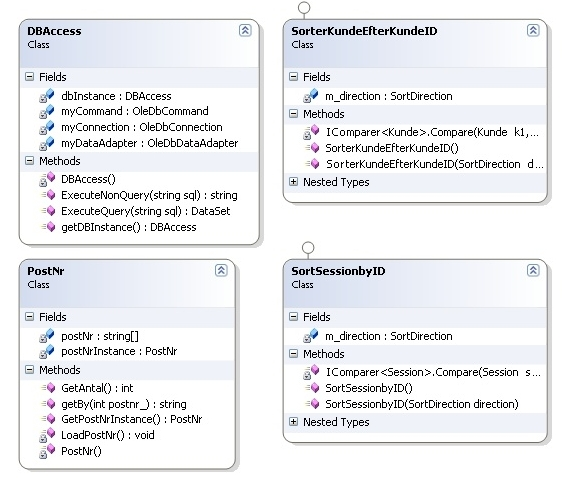
\includegraphics[width=1.00\textwidth]{Billeder/Klassediagram/ClassDiagramMiscdetaile.jpg}
	\caption{Klassediagram, Diverse}
	\label{fig:ClassDiagramMiscdetaile}
\end{figure}

Til sidst vil vi vise de mange af samme diagram, men denne gang med detailer som medlemsvariabler og -metoder.

\begin{figure}
	\centering
		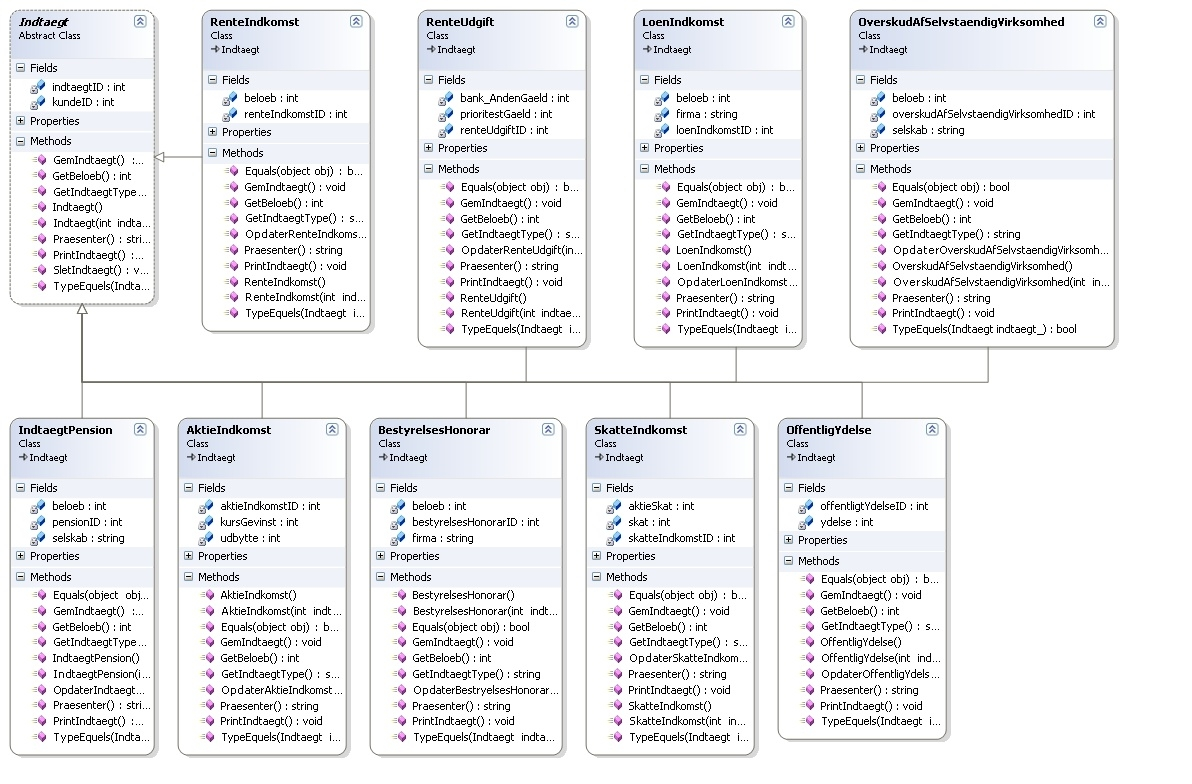
\includegraphics[angle=270, width=1.00\textwidth]{Billeder/Klassediagram/ClassDiagramIndtaegtDetaile.jpg}
	\caption{Klassediagram, Intaegt detailer}
	\label{fig:ClassDiagramIndtaegtDetaile}
\end{figure}

\begin{figure}
	\centering
		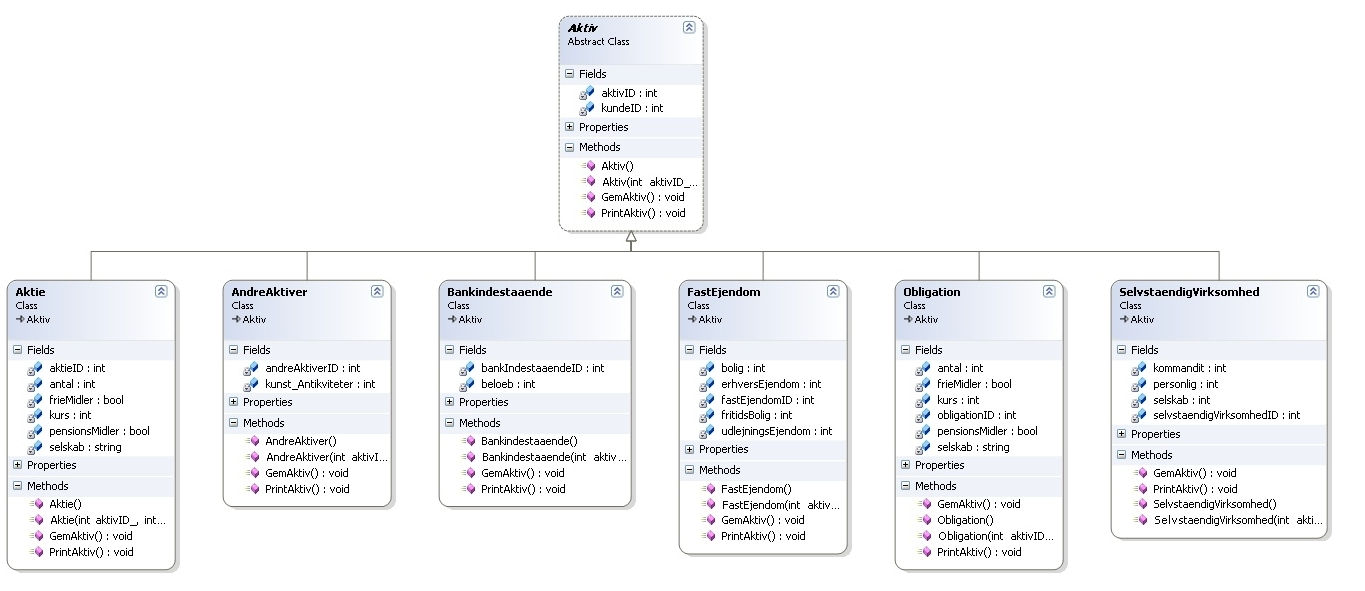
\includegraphics[angle=270, width=0.70\textwidth]{Billeder/Klassediagram/ClassDiagramAktivDetaile.jpg}
	\caption{Klassediagram, Aktiv detailer}
	\label{fig:ClassDiagramAktivDetaile}
\end{figure}

\begin{figure}
	\centering
		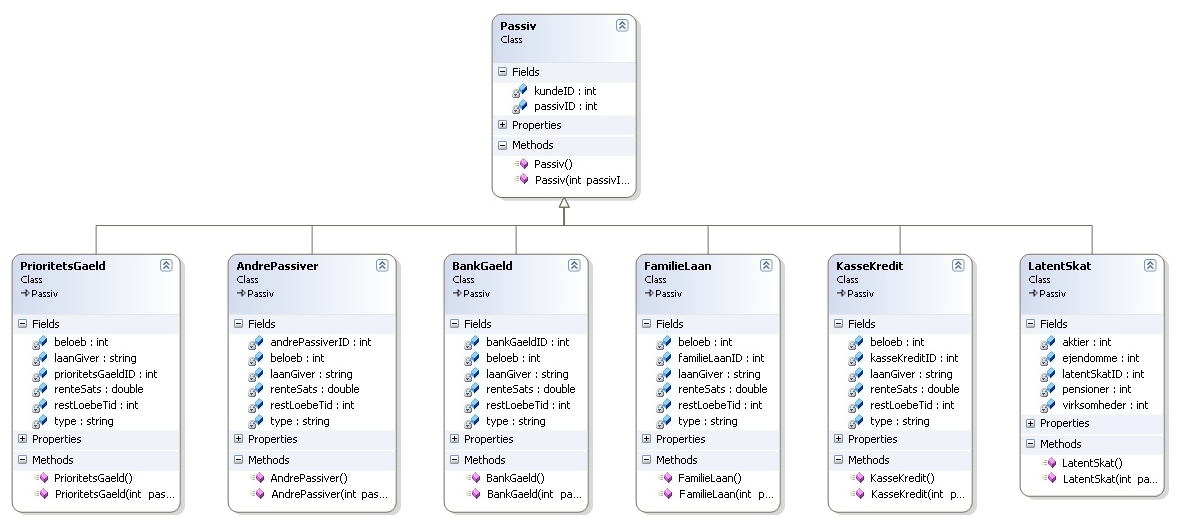
\includegraphics[angle=270, width=0.70\textwidth]{Billeder/Klassediagram/ClassDiagramPassivDetaile.jpg}
	\caption{Klassediagram, Passiv detailer}
	\label{fig:ClassDiagramPassivDetaile}
\end{figure}

\begin{figure}
	\centering
		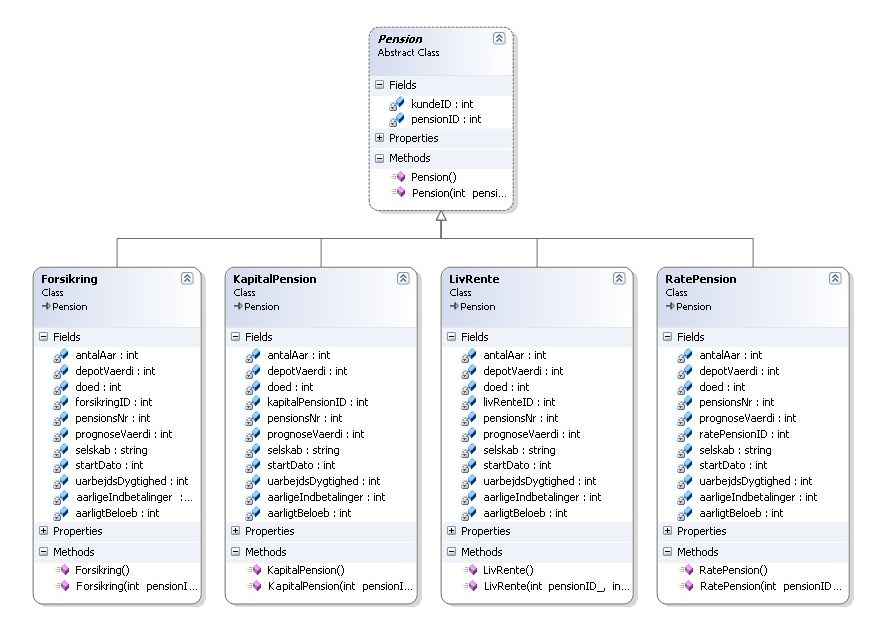
\includegraphics[angle=270, width=0.90\textwidth]{Billeder/Klassediagram/ClassDiagramPensionDetaile.jpg}
	\caption{Klassediagram, Pension detailer}
	\label{fig:ClassDiagramPensionDetaile}
\end{figure}
